\documentclass[11pt]{article}
\usepackage[sort]{natbib}
\usepackage{bm,amsmath,bbm,amsfonts,nicefrac,latexsym,amsmath,amsfonts,amsbsy,amscd,amsxtra,amsgen,amsopn,bbm,amsthm,amssymb,graphicx}
\usepackage{fancyhdr}
\usepackage[margin=1.0in]{geometry}
\usepackage[section]{placeins}
\bibliographystyle{abbrvnat}

\title{Thesis Introduction}
\author{Ewan Pinnington}

\newtheorem{theorem}{Theorem}[section]
\newtheorem*{defn}{Definition}


\begin{document}

\maketitle

\section{Notation}
List of symbols and meanings consistent throughout thesis.

\section{The global carbon cycle} \label{sec:global_c_cycle}

Carbon is one of the most abundant elements, making up around half of all living dry mass. The global carbon cycle describes the movement of carbon through the Earth system. In the Earth system large amounts of carbon are present in the oceans, atmosphere, land surface and crust. These stores of carbon are referred to as reservoirs or pools. The amount of carbon in this system can be considered constant, as under terrestrial conditions nuclear transmutation is not common. Therefore terrestrial processes using carbon must transfer it between the global carbon pools, this is referred to as a flux. In pre-industrial times the fluxes of carbon between different pools and atmospheric concentration has varied over long time scales (\(\sim\)100000 years) \citep{luthi2008high}.

The greenhouse gas effect describes the process by which radiatively active gases (CO\(_{2}\), water vapour, ozone, etc.) in the Earth's atmosphere contribute to the warming of the planet by absorbing long-wave radiation emitted from the Earth's surface and reradiating this absorbed energy in all directions, causing more warming below \citep{mitchell1989greenhouse}. The natural greenhouse gas effect raises the global mean surface temperature by 30K, making the Earth habitable for the many lifeforms upon it. The increase in atmospheric greenhouse gases since the industrial revolution due to anthropogenic activities, has amplified the greenhouse effect and caused global warming. CO\(_{2}\) has been found to be the most important human-contributed compound to this warming \citep{Falkowski291}. In figure~\ref{fig:ipcc_fig6.1} we show a simplified schematic of the global carbon cycle taken from the fifth Intergovernmental Panel on Climate Change (IPCC) report, in this schematic we can see the large rise in atmospheric CO\(_{2}\) since the industrial revolution up to 2011, with an increase of 240 Pg C.

As atmospheric CO\(_{2}\) levels have risen, natural sinks of CO\(_{2}\) (fluxes out of the atmosphere) have intensified with both the land surface and oceans absorbing more CO\(_{2}\) from the atmosphere. This can be see in figure~\ref{fig:ipcc_fig6.1}, with the the net ocean flux of CO\(_{2}\) to the atmosphere decreasing from an estimated +0.7~Pg~C~yr\(^{-1}\) to -2.3~Pg~C~yr\(^{-1}\), and the land surface flux of CO\(_{2}\) to the atmosphere decreasing from -1.7~Pg~C~yr\(^{-1}\) to -2.6~Pg~C~yr\(^{-1}\). More recent estimates from \citet{le2015global} indicate these sinks have further intensified with the ocean sink estimated to be 2.9 \(\pm 0.5\)~Pg~C~yr\(^{-1}\) and the land surface sink 4.1 \(\pm 0.9\)~Pg~C~yr\(^{-1}\) for the year 2014. The intensification of the land carbon sink is thought to be partly due to a combination of forest regrowth as well as rising CO\(_{2}\) and increased nitrogen deposition having a fertilisation effect \citep{ciais2014carbon}. It has also been shown that the land surface sink has been enhanced by an increase in diffuse photosynthetically active radiation as a result of increased cloud cover associated with increased anthropogenic emissions \citep{Mercadodiffuseradiation2009}. 

The partitioning of these fluxes of carbon between emissions and sinks is important, however current estimates are subject to high levels of uncertainty. This can be seen by the error on current estimates in Figure~\ref{fig:ipcc_fig6.1}. In Figure~\ref{fig:ipcc_fig6.8} current estimates to this partitioning are shown. It is vitally important to understand the response of sinks of CO\(_{2}\) (land surface and oceans) to climate change in the future. If either the oceans or land surface were to stop absorbing this same percentage of CO\(_{2}\) from the atmosphere, we would see even more dramatic increases in atmospheric CO\(_{2}\) levels and thus a much greater rate of global warming. \citet{1748-9326-7-2-024002} have shown that global warming is highly sensitive to land surface carbon cycle processes in particular, and highlighted the need to improve understanding of land surface carbon uptake and its response to climate change. There is a high level of confidence that ocean carbon uptake will continue under all future emission scenarios. Land surface carbon uptake is much more uncertain with some estimates showing the land surface changing from a sink of CO\(_{2}\) to a source of CO\(_{2}\) under certain future emission scenarios \citep{sitch2008evaluation, cox2000}.

\begin{figure}[ht]
    \centering
    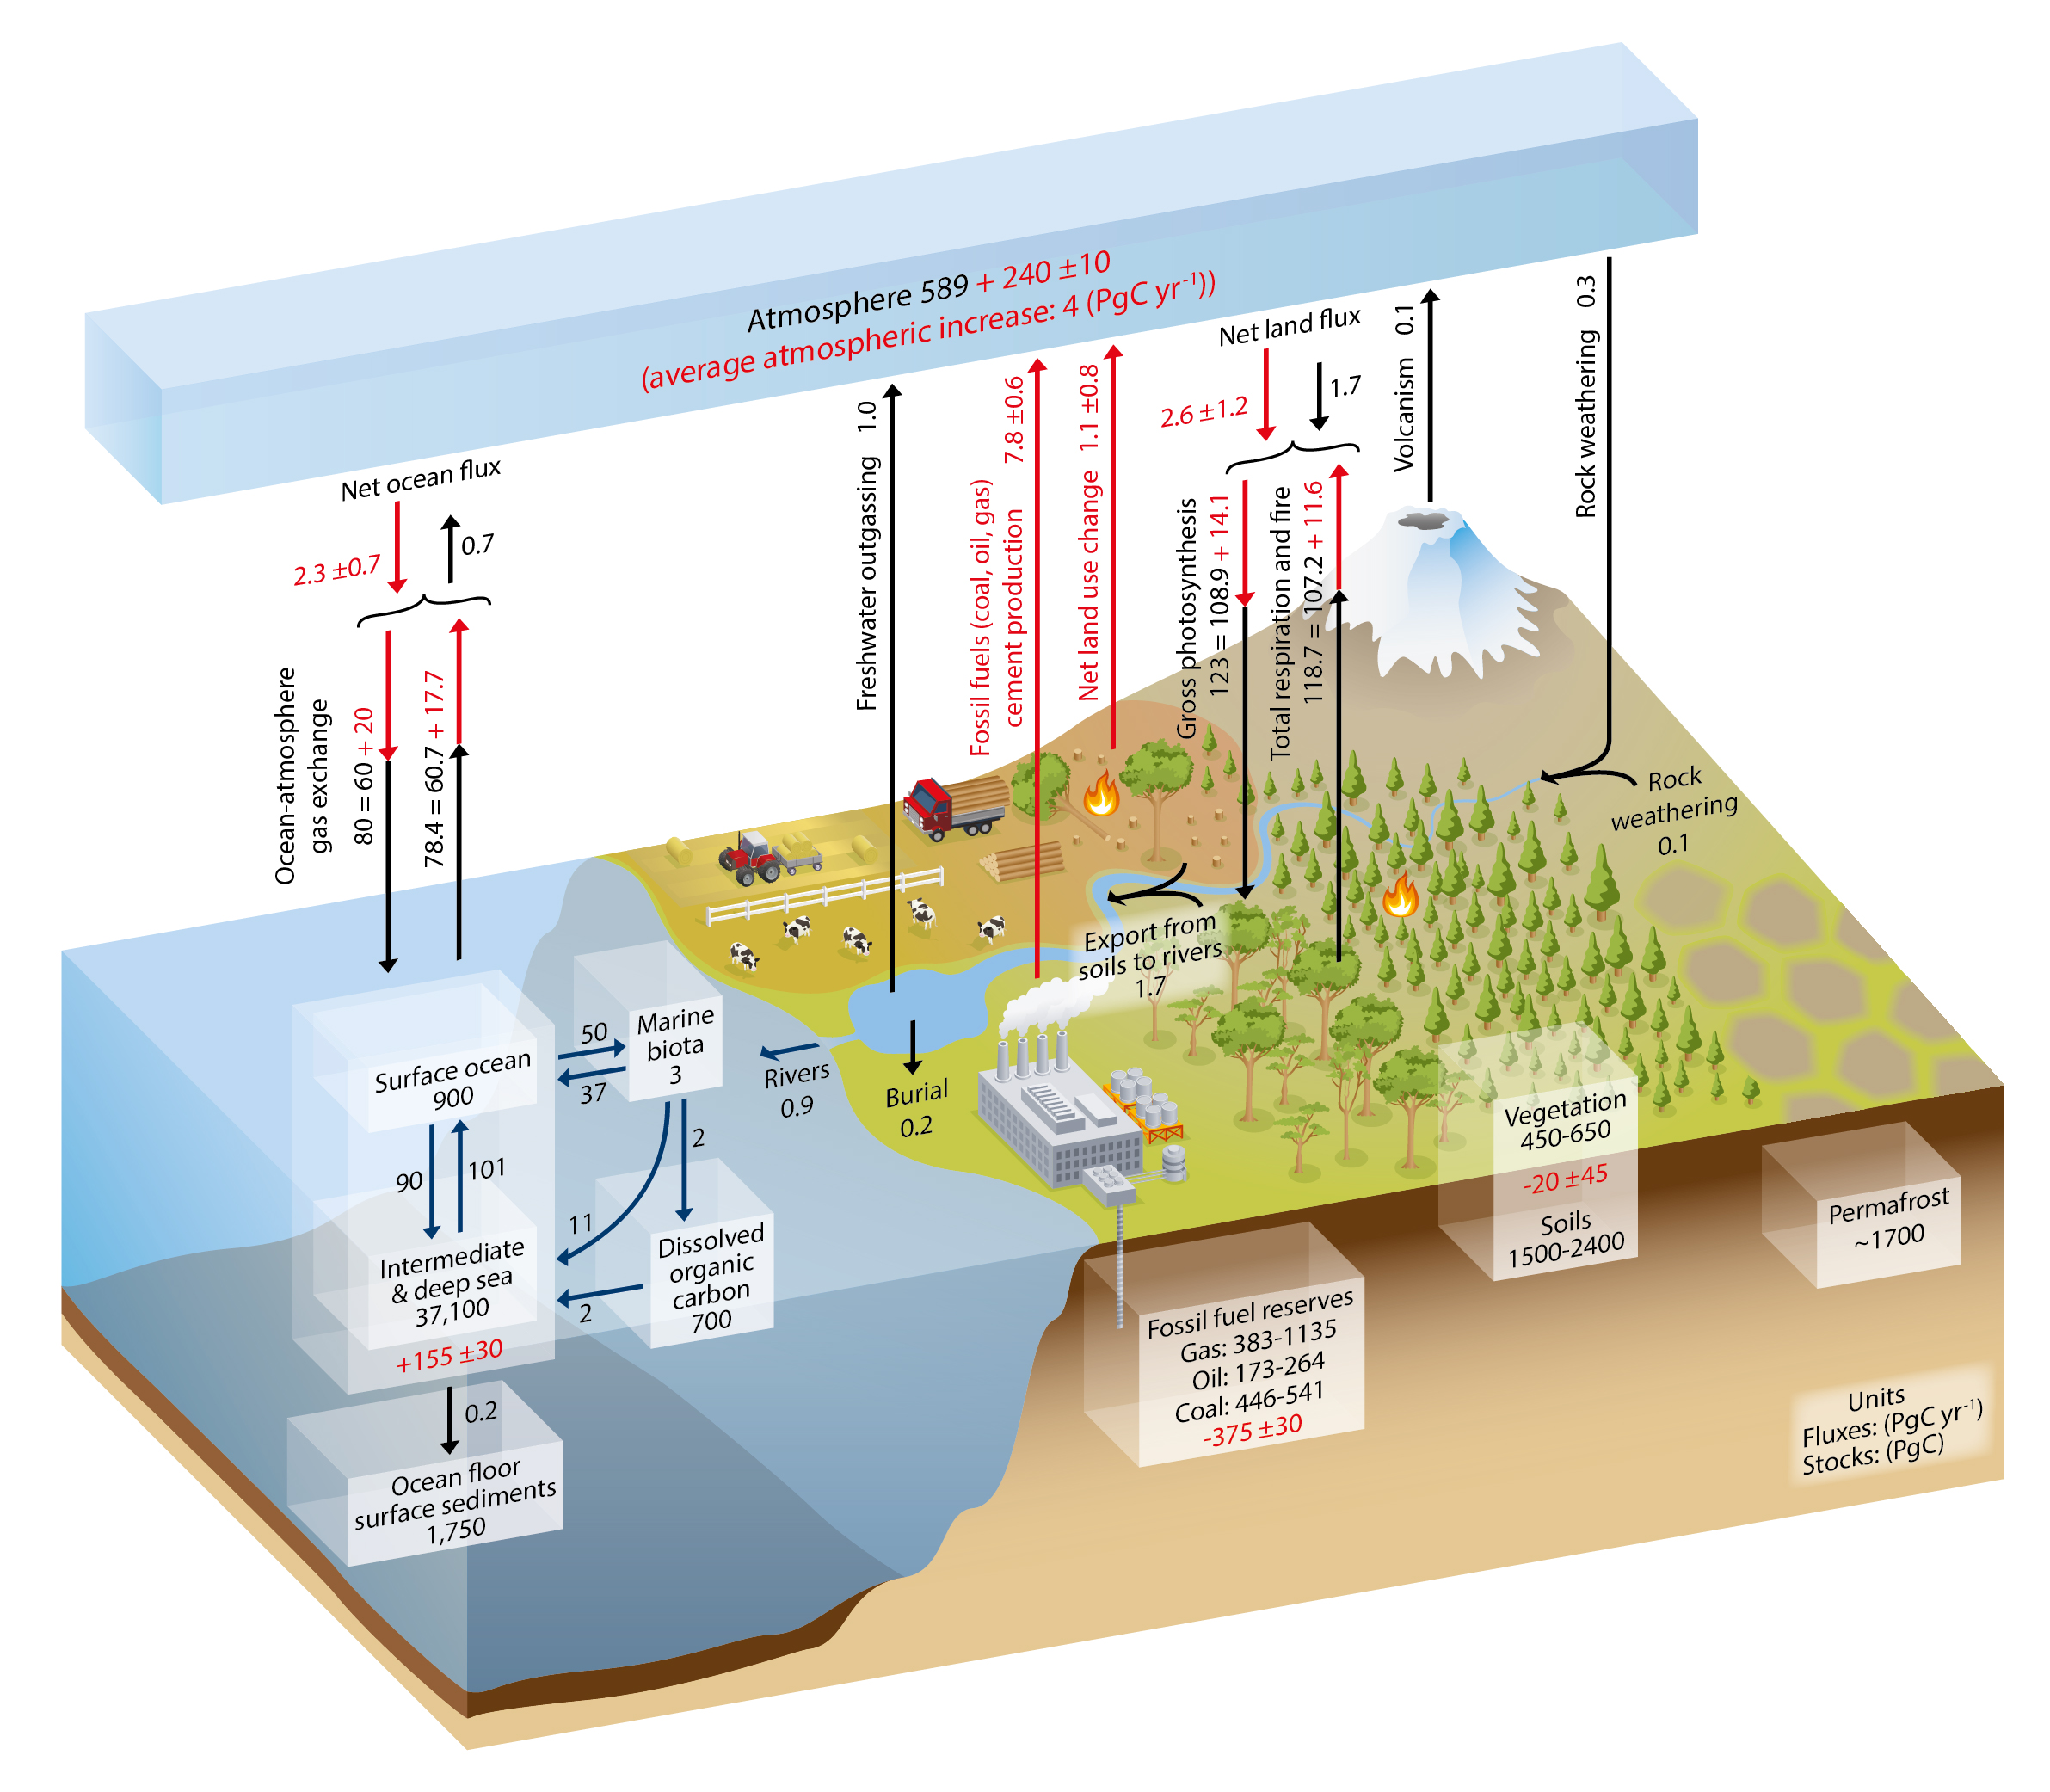
\includegraphics[width=0.6\textwidth]{ipcc_fig6_1.jpg}
    \caption{Global carbon cycle simplified schematic \citep{ciais2014carbon}. Black numbers and arrows represent reservoir mass and exchange fluxes estimated for the time prior to the industrial era (\(\sim\)~1750). Red numbers and arrows represent annual fluxes average over the 2000-2009 time period. Red numbers in the reservoirs indicate the cumulative change of carbon over the industrial period (1750-2011).}
    \label{fig:ipcc_fig6.1}
\end{figure}

Land surface carbon uptake is the least understood process in the global carbon cycle \citep{ciais2014carbon}, this can be seen in the uncertainties given in Figure~\ref{fig:ipcc_fig6.1}. In current estimates of the global carbon budget, land surface carbon uptake is estimated by taking the residual of all other calculated sources and sinks of carbon, so that
\begin{equation}
S_{LAND} = E_{FF} + E_{LUC} - (G_{ATM} + S_{OCEAN})
\end{equation}  
where \(S_{LAND}\) is the global residual land sink of CO\(_{2}\), \(E_{FF}\) is the CO\(_{2}\) emissions from fossil fuels, \(E_{LUC}\) is the CO\(_{2}\) emissions from land use change (mainly deforestation), \(G_{ATM}\) is the atmospheric CO\(_{2}\) growth rate and \(S_{OCEAN}\) is the mean ocean CO\(_{2}\) sink \citep{le2015global}. In Figure~\ref{fig:ipcc_fig6.8} we can see the growth in this residual land sink with increased emissions, it can also be seen that there is a high variability in this sink, largely due to year to year variations in precipitation, surface temperature, radiation and volcanic eruptions.

Land use change is the next most uncertain component in the global carbon cycle and the second largest anthropogenic source of CO\(_{2}\). It is not well understood how much CO\(_{2}\) is removed from the atmosphere by regrowth of previously deforested land (either by felling or fire), although it is thought that regrowth forests could be stronger carbon sinks than old growth forests, due to more rapid biomass accumulation under succession \citep{pan2011large}. Better understanding the response of the land surface to disturbance will help constrain future carbon budgets. 

%Good paper to highlight the fact that the percentage of CO\(_{2}\) absorbed by the land surface has remained approximately constant with rising atmospheric CO\(_{2}\) levels??? Maybe just use IPCC fig 6.8?

%In figure 6.1 and 6.8: Partitioning of fluxes important and hard (shown by error on estimates in fig 6.1). Land surface carbon uptake least understood mechanism in the global carbon cycle, ref IPCC. Will uptake remain the same under climate change.

%Human emissions of CO\(_{2}\) have perturbed the global C cycle and caused a large continual increase in atmospheric CO\(_{2}\) levels.

%Look at papers recommended on Flux Course, some good ones to reference???

\begin{figure}[ht]
    \centering
    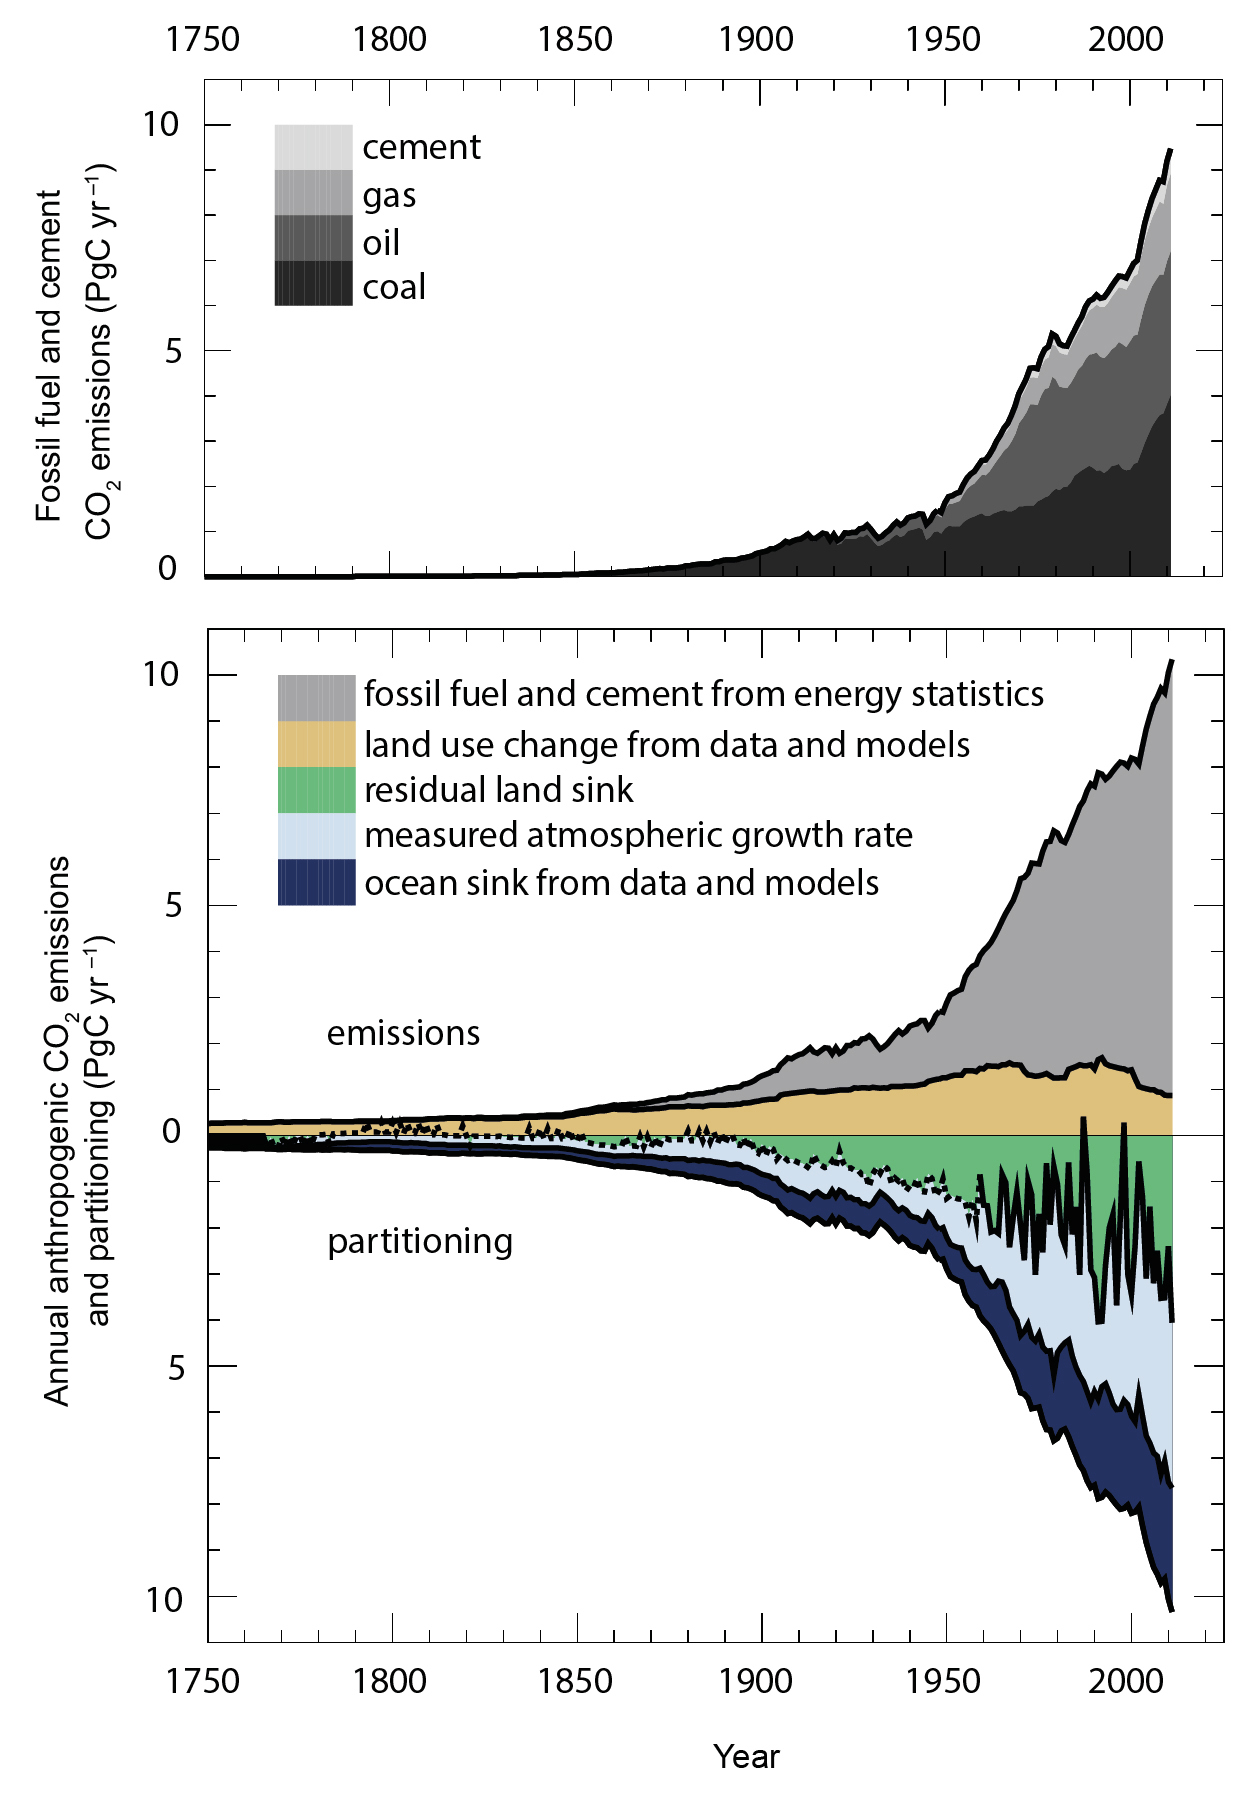
\includegraphics[width=0.6\textwidth]{ipcc_fig6_8.jpg}
    \caption{Annual anthropogenic CO\(_{2}\) emissions and their partitioning among the atmosphere, land and ocean from 1750 to 2011  \citep{ciais2014carbon}.}
    \label{fig:ipcc_fig6.8}
\end{figure}

%IPCC figure 6.1 and 6.8: Partitioning of fluxes important and hard (shown by error on estimates in fig 6.1). Land surface carbon uptake least understood mechanism in the global carbon cycle, ref IPCC. Will uptake remain the same under climate change.

%\citet{1748-9326-7-2-024002} Have shown that global warming is highly sensitive to land carbon cycle processes and highlighted the need to improve understanding of land surface carbon uptake and its response to climate change. 

\section{Observations of terrestrial carbon balance}

There are an increasing number of available observations relevant to understanding the carbon balance of forests and the terrestrial biosphere. These observations are of a range of variables, perhaps two of the most common are the Net Ecosystem Exchange (NEE) of CO\(_{2}\), which is equal to the difference between photosynthesis and respiration, and Leaf Area Index (LAI) which is the area of leaves per unit area ground. These variables can be directly measured at site level and also estimated from remotely sensed satellite products.

%para on flux network and site level data:
At site level some of the most valuable information comes from flux tower sites measuring ecosystem-atmosphere fluxes of CO\(_{2}\), water and energy using the method of eddy covariance. From these flux towers we have direct observations of ecosystem CO\(_{2}\) uptake at a fine temporal resolution, with observations made every half-hour. In recent years there has been a growing number of flux tower sites implemented, with many of these sites forming part of the global flux network FLUXNET, which was established in 1997 \citep{baldocchi2001fluxnet}. The current active FLUXNET sites are shown in Figure~\ref{fig:fluxnet_2015}; we can see that although there are 517 sites, these sites are not well distributed spatially, it is therefore not possible to use FLUXNET sites alone to produce global estimates of terrestrial CO\(_{2}\) balance. However, these sites do provide an invaluable resource for model and satellite calibration which can then in turn be used to produce estimates on a global scale. At many flux tower sites and forest stands other diverse observations relevant to terrestrial carbon budgets are also being made. These include observations of soil and litter respiration, woody biomass and LAI, with many of these observations being made much less frequently than flux tower observations of ecosystem CO\(_{2}\) exchange as they are labour intensive.     

\begin{figure}[ht]
\centering
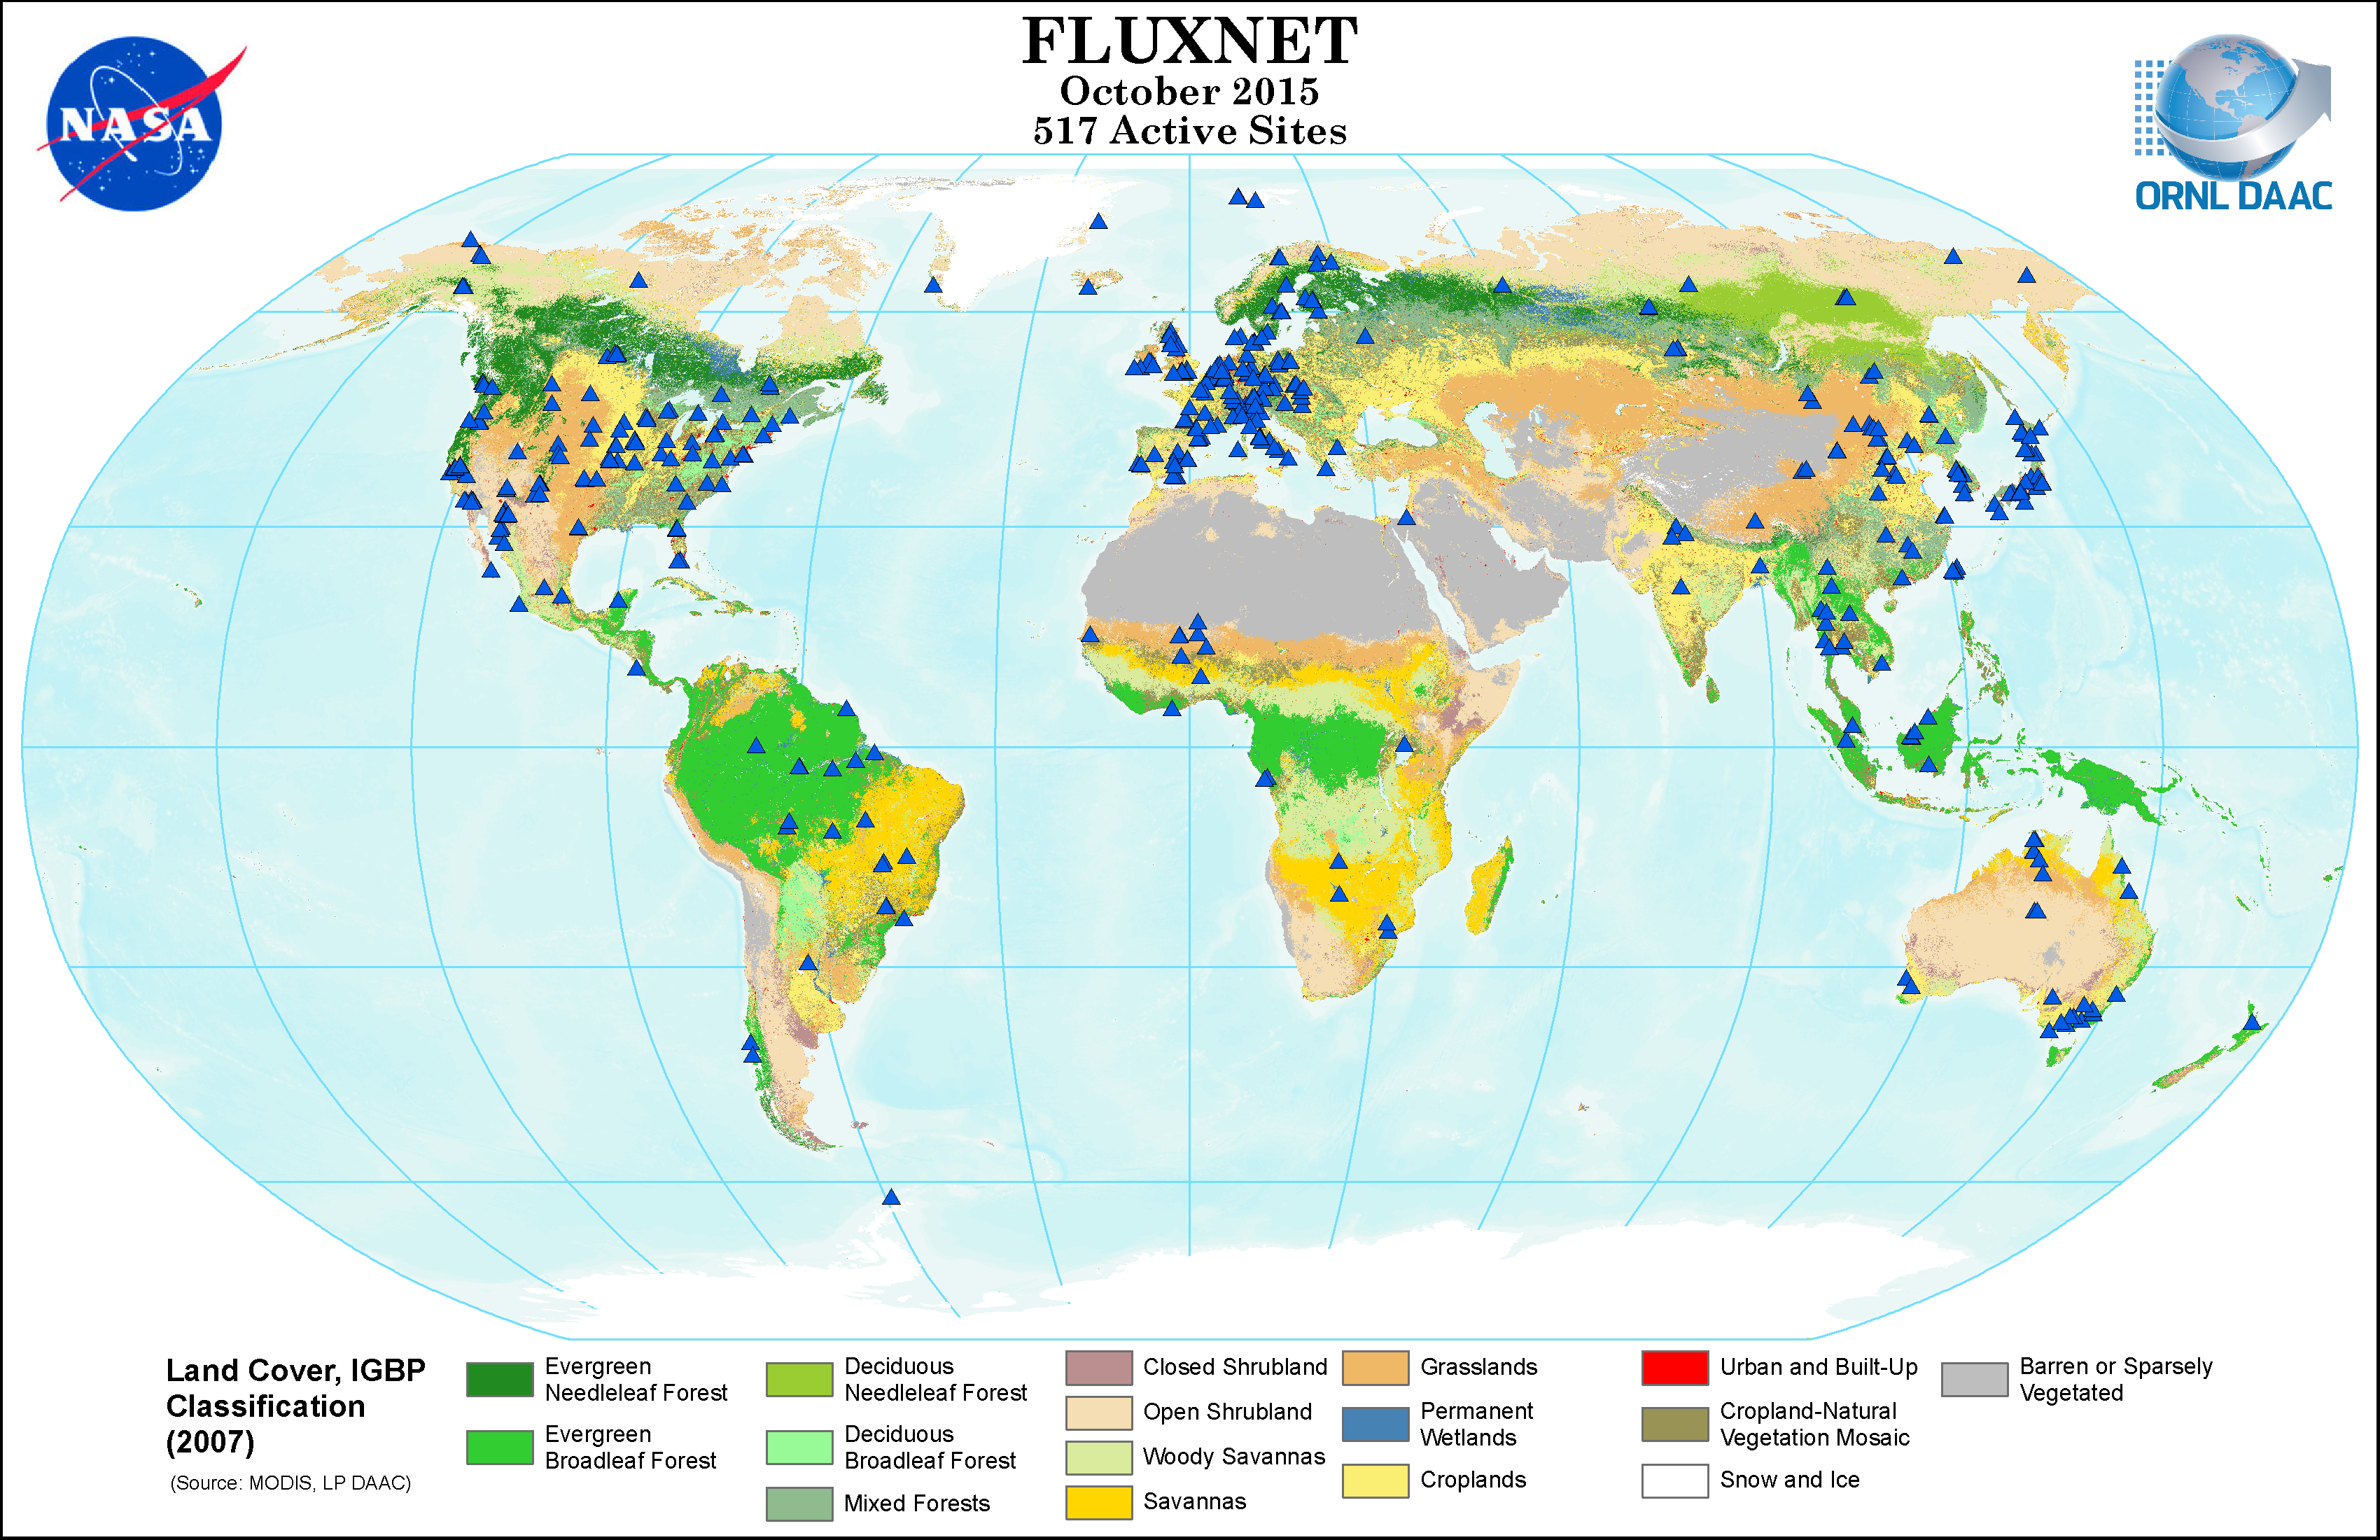
\includegraphics[width=0.9\textwidth]{FluxNetworkMODIS_IGBP_10-2015.png}
\caption{FLUXNET sites and land cover (MODIS IGBP classification) \citep{fluxnetsite2013}.}
\label{fig:fluxnet_2015}
\end{figure}

%para on satellite data
The Moderate Resolution Imaging Spectroradiometer (MODIS) on the TERRA and AQUA satellites produces global estimates to LAI and Gross Primary Productivity (GPP) for terrestrial ecosystems \citep{running2004continuous}. These estimates are derived by converting the remotely sensed reflected sunlight to vegetation indices, such as the Normalised Difference Vegetation Index (NDVI) and then correlating these indices with the fraction of absorbed visible sunlight for LAI or using these indices in simple algorithms for GPP \citep{yuan2007deriving}. For LAI it has been shown that remotely sensed estimates saturate when measuring ecosystems with a LAI above 3 \citep{myneni2002global}. Terrestrial fluxes of carbon estimated from satellite measurements are subject to large errors in representativity, as satellites view a scene almost instantaneously and then derive daily mean fluxes \citep{baldocchi2008turner}. 
%Baldocchi paper: Many observations of forest carbon flux made worldwide.

\section{The role of models}

Observations can only tell us about the current and past state of a system. In order to produce future predictions and better understand current terrestrial carbon dynamics we must use mathematical models. Figure~\ref{fig:ipcc_fig6.16} show a comparison of the residual land sink (described in section~\ref{sec:global_c_cycle}) with the global terrestrial CO\(_{2}\) sink estimated from different process based global carbon cycle models. We see that although there is a high variability between modelled estimates there is good agreement between the multi-model mean and the residual land sink. 

\begin{figure}[ht]
    \centering
    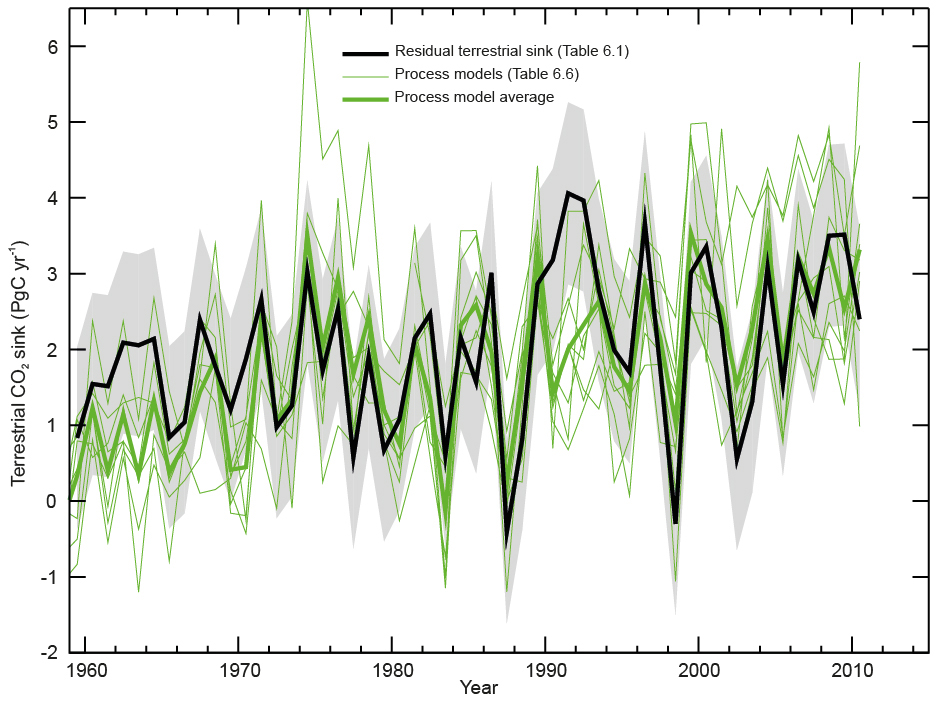
\includegraphics[width=0.9\textwidth]{ipcc_fig6_16.jpg}
    \caption{Comparison of the residual land sink with the global terrestrial CO\(_{2}\) sink estimated from different process based global carbon cycle models \citep{ciais2014carbon}.}
    \label{fig:ipcc_fig6.16}
\end{figure}

Future model predictions of terrestrial carbon uptake based on Representative Concentration Pathways (RCPs) \citep{moss2010next} of CO\(_{2}\) concentrations and emissions are highly uncertain with little agreement between different process based models. Under these different emission scenarios some models predicted the land surface to become a source of CO\(_{2}\) and others predicted a further intensification of the residual land sink \citep{jones2013twenty}. In comparison model predictions of future ocean carbon uptake have a much higher level of agreement and reduced uncertainty. This large uncertainty for terrestrial carbon models is in part due to poor model parameterisations and missing processes within models. One of the main processes many current global models do not account for is the effect of disturbances on terrestrial ecosystem carbon dynamics. Disturbance can come from many different sources such as; fire, human management and insect outbreaks.

In order to improve global models of terrestrial carbon balance it is important to improve processes and parameterisations of models at site-level where we have diverse sets of direct observations with which to judge model performance.         

%IPCC figure 6.16 and section 6.3.2.6.6: Contribution of models to understanding the terrestrial carbon cycle. Reference every DALEC paper.


\section{Data assimilation}

Role of DA in NWP improving forecast skill. 


\bibliography{../PhD}{}
\end{document}